\documentclass[aspectratio=169]{beamer}

\mode<presentation>
{
  \usetheme{default}
  \usecolortheme{default}
  \usefonttheme{default}
  \setbeamertemplate{navigation symbols}{}
  \setbeamertemplate{caption}[numbered]
  \setbeamertemplate{footline}[frame number]  % or "page number"
  \setbeamercolor{frametitle}{fg=white}
  \setbeamercolor{footline}{fg=black}
} 

\usepackage[english]{babel}
\usepackage[utf8x]{inputenc}
\usepackage{tikz}
\usepackage{courier}
\usepackage{array}
\usepackage{bold-extra}
\usepackage{minted}
\usepackage[thicklines]{cancel}
\usepackage{fancyvrb}

\xdefinecolor{dianablue}{rgb}{0.18,0.24,0.31}
\xdefinecolor{darkblue}{rgb}{0.1,0.1,0.7}
\xdefinecolor{darkgreen}{rgb}{0,0.5,0}
\xdefinecolor{darkgrey}{rgb}{0.35,0.35,0.35}
\xdefinecolor{darkorange}{rgb}{0.8,0.5,0}
\xdefinecolor{darkred}{rgb}{0.7,0,0}
\definecolor{darkgreen}{rgb}{0,0.6,0}
\definecolor{mauve}{rgb}{0.58,0,0.82}

\title[2018-07-12-chep-plenary-datamodels]{Evolution of data models, formats, and analysis}
\author{Jim Pivarski}
\institute{Princeton University -- DIANA-HEP}
\date{July 12, 2018}

\begin{document}

\logo{\pgfputat{\pgfxy(0.11, 7.4)}{\pgfbox[right,base]{\tikz{\filldraw[fill=dianablue, draw=none] (0 cm, 0 cm) rectangle (50 cm, 1 cm);}\mbox{\hspace{-8 cm}
\includegraphics[height=1 cm]{princeton-logo-long.png}
\includegraphics[height=1 cm]{diana-hep-logo-long.png}}}}}

\begin{frame}
  \titlepage
\end{frame}

\logo{\pgfputat{\pgfxy(0.11, 7.4)}{\pgfbox[right,base]{\tikz{\filldraw[fill=dianablue, draw=none] (0 cm, 0 cm) rectangle (50 cm, 1 cm);}\mbox{\hspace{-8 cm}
\includegraphics[height=1 cm]{princeton-logo.png}
\includegraphics[height=1 cm]{diana-hep-logo.png}}}}}

% Uncomment these lines for an automatically generated outline.
%\begin{frame}{Outline}
%  \tableofcontents
%\end{frame}

% START START START START START START START START START START START START START

\begin{frame}{}
\Large
\vspace{0.5 cm}
\begin{center}
I'm going to start with a dumb comparison, to make a point.
\end{center}
\end{frame}

\begin{frame}{\only<1>{We measure globally distributed data in hundreds of PB}\only<2>{But for ``web scale'' companies, 100 PB = 1 truck}}
\vspace{0.35 cm}
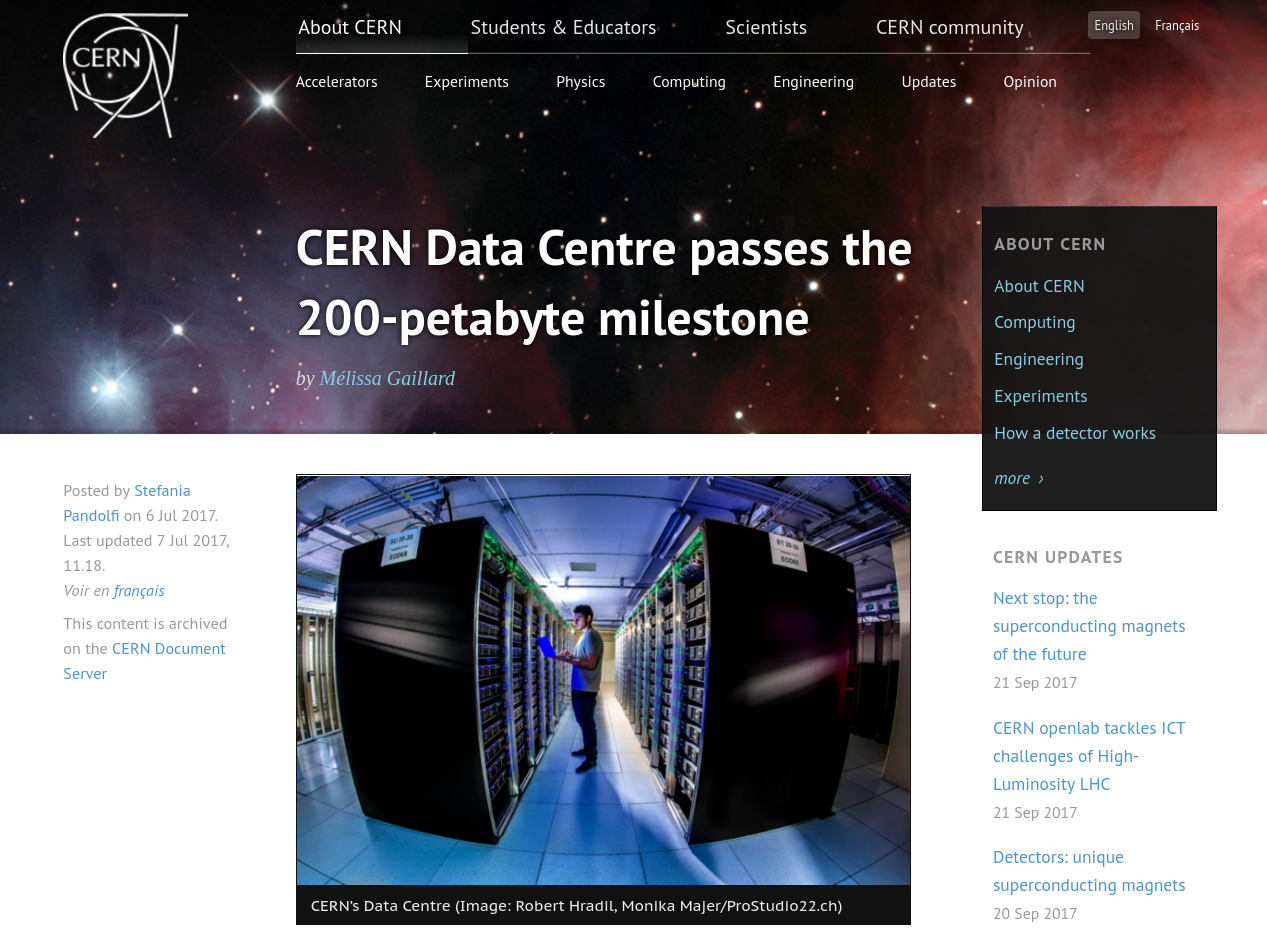
\includegraphics[width=0.73\linewidth]{cern-200pb.png}

\vspace{-4.8 cm}
\uncover<2->{\mbox{ } \hfill 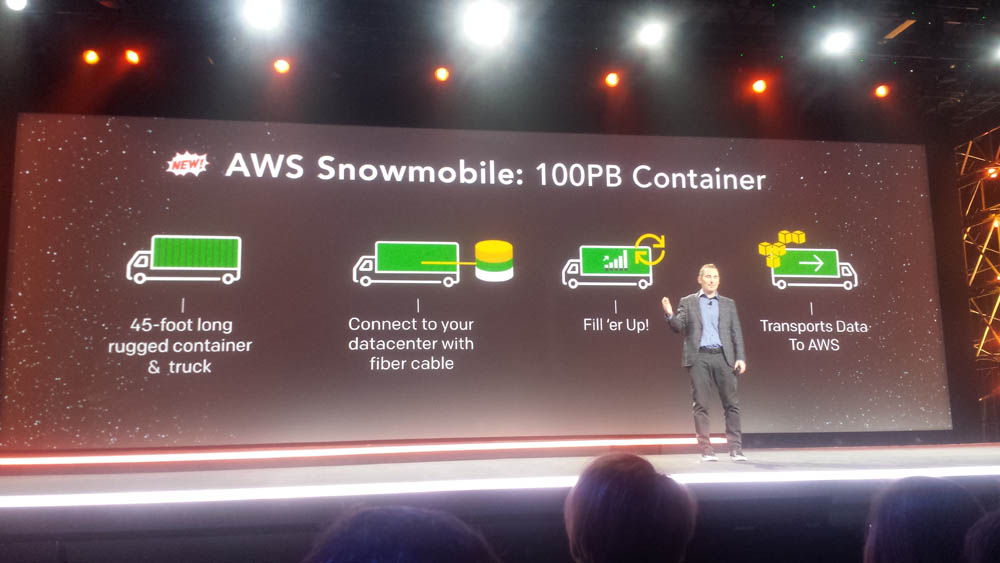
\includegraphics[width=0.7\linewidth]{aws-snowmobile.jpg}\hspace{-1 cm}}
\end{frame}

\begin{frame}{The point?}
\Large
\vspace{0.5 cm}
HEP is no longer the main user or developer in this problem space.

\vspace{1 cm}
\begin{uncoverenv}<2->
A better metric, which unfortunately I can't quantify:
\begin{itemize}
\item $x$~FTEs in HEP developing open source analysis tools
\item $y$~FTEs outside of HEP developing open source analysis tools
(not sure of $x$ and $y$, but $x \ll y$)
\end{itemize}
\end{uncoverenv}

\vspace{0.5 cm}
\uncover<3->{$\to$ there's a lot of good data analysis software out there!}
\end{frame}

\begin{frame}{Another very important metric}
\Large
\vspace{0.25 cm}
\begin{itemize}
\item High-energy physicists have been performing big data analytics (i.e.\ reducing large datasets to statistical inferences with computers) for about \textcolor{darkblue}{\underline{50~years}.}
\item<2-> Web-scale companies have been doing it for about \textcolor{darkblue}{\underline{10~years}.}
\end{itemize}

\vspace{0.5 cm}
\uncover<3->{HEP analyses have grown sophisticated--- there are certain things we expect but don't find in industry-grade software.}

\vspace{0.5 cm}
\uncover<4->{The simple prescription of ``just use Spark'' would leave analyzers}

\vspace{0.2 cm}
\uncover<4->{without some necessary tools.}
\end{frame}

\begin{frame}{Reactions?}
\large
\vspace{0.5 cm}
\begin{columns}[t]
\column{0.25\linewidth}
\textcolor{darkblue}{\underline{Option \#1}}

\vspace{0.25 cm}
Our needs are very specific. Continue developing our own everything.

\column{0.25\linewidth}
\begin{uncoverenv}<2->
\textcolor{darkblue}{\hspace{-0.18 cm}\underline{Option \#2}}

\vspace{0.25 cm}
Modern big data software has some good ideas; integrate those \underline{\it ideas} into our stack.
\end{uncoverenv}

\column{0.25\linewidth}
\begin{uncoverenv}<3->
\only<3-4>{\textcolor{darkblue}{\hspace{-0.18 cm}\underline{Option \#3}}}\only<5->{\textcolor{red}{\hspace{-0.18 cm}\underline{Option \#3}}}

\vspace{0.25 cm}
\only<3-4>{Narrow our scope to HEP-specific tools, what no one else is developing, and make them interoperate with non-HEP tools for the common parts.}\only<5->{\textcolor{red}{Narrow our scope to HEP-specific tools, what no one else is developing, and make them interoperate with non-HEP tools for the common parts.}}
\end{uncoverenv}

\column{0.25\linewidth}
\begin{uncoverenv}<4->
\textcolor{darkblue}{\hspace{-0.18 cm}\underline{Option \#4}}

\vspace{0.25 cm}
Promulgate the HEP way of doing analysis to bring the wider world up to our level of sophistication. Then they'll develop solutions for us.
\end{uncoverenv}
\end{columns}

\vspace{1 cm}
\uncover<5->{\textcolor{red}{\#3 is my opinion, but it begs the question of where to draw the line.}}
\end{frame}

\begin{frame}{Three examples each:}
\Large
\vspace{0.5 cm}
\begin{columns}[t]
\column{0.5\linewidth}
\mbox{\hspace{0.25 cm}\underline{What they've got}}

\vspace{0.25 cm}
\begin{enumerate}
\item Distributed DAG processing
\item Indexed analysis
\item Machine learning
\end{enumerate}

\column{0.5\linewidth}
\mbox{\hspace{0.45 cm}\underline{What we'd need}}

\vspace{0.25 cm}
\begin{enumerate}
\item Nested data structures
\item Advanced histogramming
\item Ansatz fitting
\end{enumerate}

\end{columns}
\end{frame}

\begin{frame}{Distributed DAG processing}
\large
\vspace{0.5 cm}
\begin{columns}
\column{0.21\linewidth}
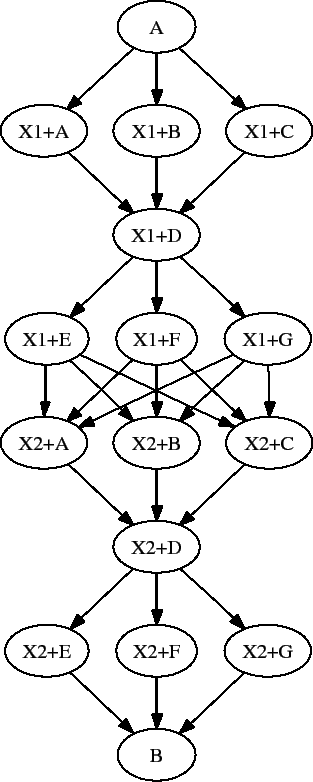
\includegraphics[width=\linewidth]{dag-htcondor.png}

\column{0.83\linewidth}
DAG: Directed Acyclic Graph of dependencies between subtasks.

In a common point of view, this is what big data processing \underline{\it is}.

\vspace{0.5 cm}
\begin{uncoverenv}<2->
Many projects distribute tasks this way:

\vspace{0.2 cm}
\hfill \begin{minipage}{0.95\linewidth}
\textcolor{darkblue}{Spark} (JVM), \textcolor{darkblue}{Dask} and \textcolor{darkblue}{Joblib} (Python), \textcolor{darkblue}{Storm} (continuous), \textcolor{darkblue}{Thrill} (C++), \textcolor{darkblue}{DAGMan} (HTCondor), \textcolor{darkblue}{TensorFlow} (ML)\ldots
\end{minipage}
\end{uncoverenv}

\vspace{0.5 cm}
\begin{uncoverenv}<3->
To use these projects, one must
\begin{itemize}
\item express user tasks as DAG nodes (e.g.\ ROOT RDataFrame)
\item serialize user functions on the driver and load user data on the workers, within the framework's environment
\end{itemize}
\end{uncoverenv}

\vspace{0.5 cm}
\begin{uncoverenv}<4->
Spectrum of solutions from ``bare Spark'' to ``reimplement Spark.''
\end{uncoverenv}
\end{columns}
\end{frame}

\begin{frame}{Distributed DAG processing}
\Large
\vspace{0.5 cm}
\begin{center}
However, most analysis needs for DAG processing are pretty simple: one level of map (embarrassingly parallel event processing) and maybe one level of reduce (combining aggregations: hadd).
\end{center}
\end{frame}

\begin{frame}{Nested data structures}
\end{frame}

\begin{frame}{Indexed analysis}
\Large
\vspace{0.5 cm}
\begin{center}
To understand what I mean by ``indexed analysis,'' consider \\
analysis with \underline{\it less advanced indexing} than modern HEP.
\end{center}
\end{frame}

\begin{frame}[fragile]{Indexed analysis}
\vspace{0.1 cm}
\begin{columns}
\column{0.5\linewidth}
\tiny
\begin{Verbatim}[commandchars=\\\{\}]
h/cr/1d \textcolor{red}{201} 'd0miss' 100 -0.5e-3 0.5e-3
h/cr/1d \textcolor{red}{202} 'z0miss' 100 -0.015 0.015
h/cr/1d \textcolor{red}{203} 'pxmiss' 100 -0.076 0.076
h/cr/1d \textcolor{red}{204} 'pymiss' 100 -0.076 0.076
h/cr/1d \textcolor{red}{205} 'pzmiss' 100 -0.076 0.076
nt/plot 2.d0 ! ! ! ! ! \textcolor{red}{201}
nt/plot 2.z0 ! ! ! ! ! \textcolor{red}{202}
nt/plot 2.px ! ! ! ! ! \textcolor{red}{203}
nt/plot 2.py ! ! ! ! ! \textcolor{red}{204}
nt/plot 2.pz ! ! ! ! ! \textcolor{red}{205}

h/cr/1d \textcolor{red}{301} 'normalized d0miss' 100 -10 10
h/cr/1d \textcolor{red}{302} 'normalized z0miss' 100 -10 10
h/cr/1d \textcolor{red}{303} 'normalized pxmiss' 100 -10 10
h/cr/1d \textcolor{red}{304} 'normalized pymiss' 100 -10 10
h/cr/1d \textcolor{red}{305} 'normalized pzmiss' 100 -10 10
nt/plot 2.d0/sqrt(ed0) ! ! ! ! ! \textcolor{red}{301}
nt/plot 2.z0/sqrt(ez0) ! ! ! ! ! \textcolor{red}{302}
nt/plot 2.px/sqrt(epx) ! ! ! ! ! \textcolor{red}{303}
nt/plot 2.py/sqrt(epy) ! ! ! ! ! \textcolor{red}{304}
nt/plot 2.pz/sqrt(epz) ! ! ! ! ! \textcolor{red}{305}

h/cr/1d \textcolor{red}{401} 'd0miss after constraint' 100 -0.1e-16 0.1e-16
h/cr/1d \textcolor{red}{402} 'z0miss after constraint' 100 -0.1e-15 0.1e-15
h/cr/1d \textcolor{red}{403} 'pxmiss after constraint' 100 -0.01 0.01
h/cr/1d \textcolor{red}{404} 'pymiss after constraint' 100 -0.01 0.01
h/cr/1d \textcolor{red}{405} 'pzmiss after constraint' 100 -0.01 0.01
nt/plot 2.ad0 ! ! ! ! ! \textcolor{red}{401}
nt/plot 2.az0 ! ! ! ! ! \textcolor{red}{402}
nt/plot 2.apx ! ! ! ! ! \textcolor{red}{403}
nt/plot 2.apy ! ! ! ! ! \textcolor{red}{404}
nt/plot 2.apz ! ! ! ! ! \textcolor{red}{405}
\end{Verbatim}

\column{0.01\linewidth}

\column{0.5\linewidth}
To the left is a PAW script (pre-ROOT), creating and filling histograms.

\vspace{0.75 cm}
\textcolor{red}{They must be identified by integers because histograms didn't have \underline{\it names} back then.}

\vspace{0.75 cm}
\uncover<2->{{\bf Acquiring the ability to name stuff was as fundamental to HEP data analysis as handwashing was to medical science!}}

\vspace{0.75 cm}
\uncover<3->{But we don't have to stop there. There's more to indexing than key-value pairs.}
\end{columns}
\end{frame}

\begin{frame}{From ``Pandas DataFrames for F.A.S.T.\ binned analysis at CMS''}
\begin{center}
\only<1>{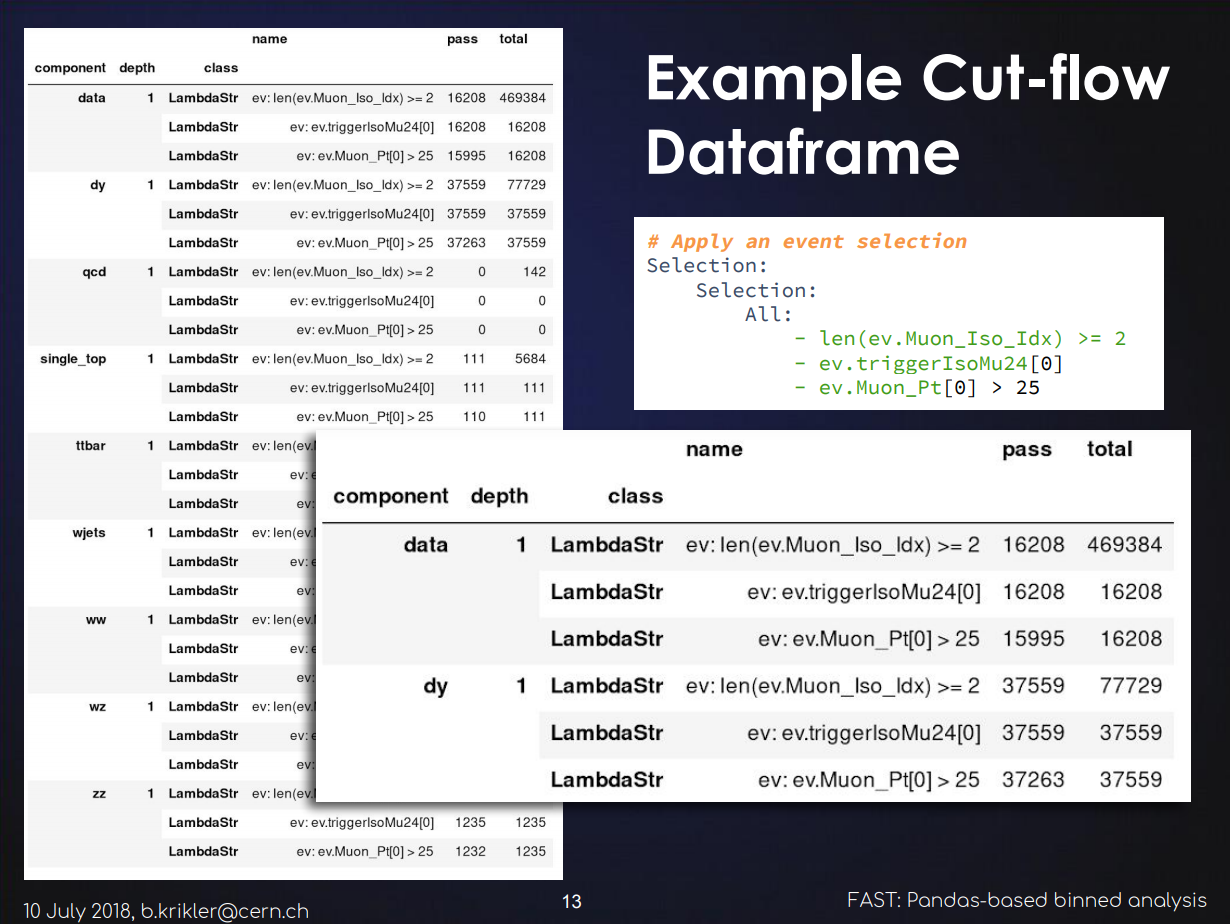
\includegraphics[width=0.75\linewidth]{fast-slide-0.png}}\only<2>{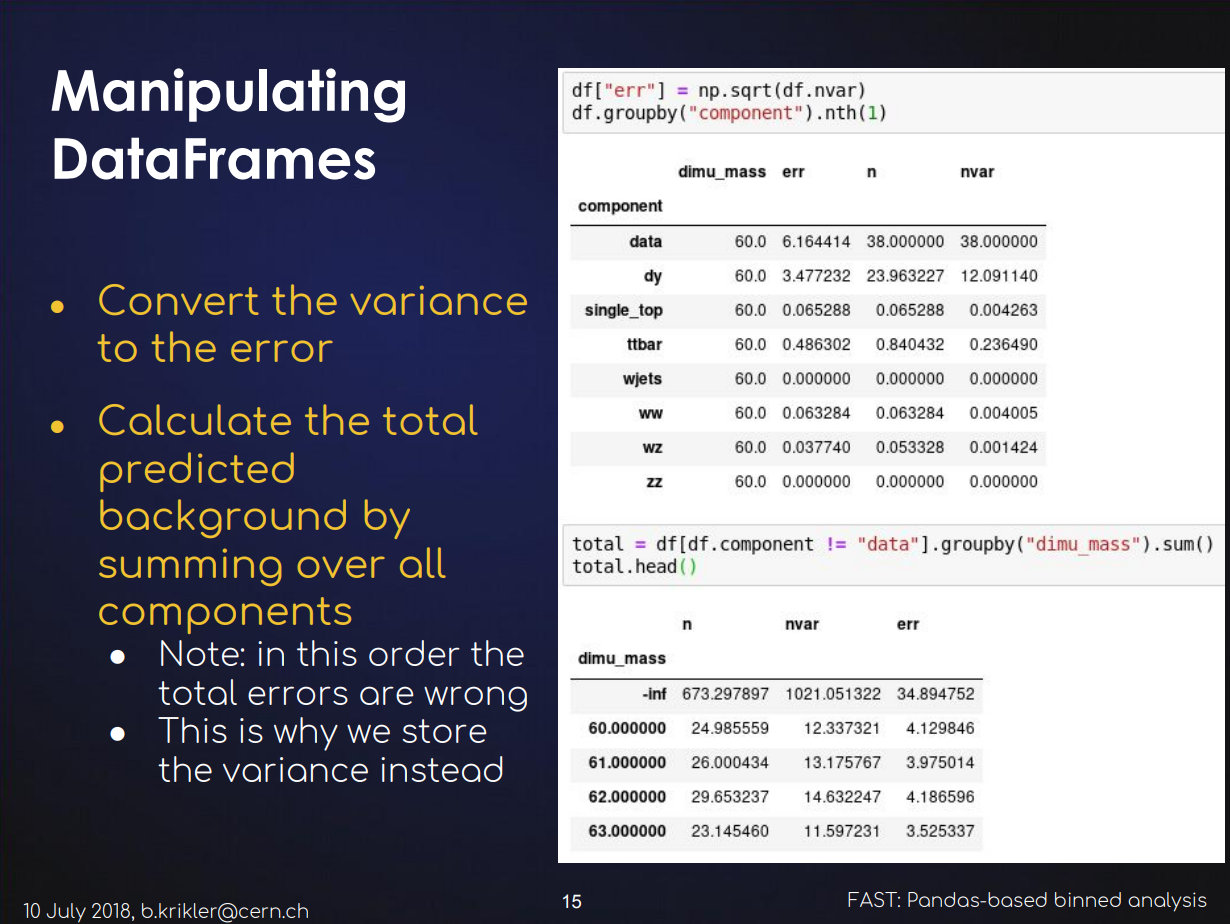
\includegraphics[width=0.75\linewidth]{fast-slide-1.png}}\only<3>{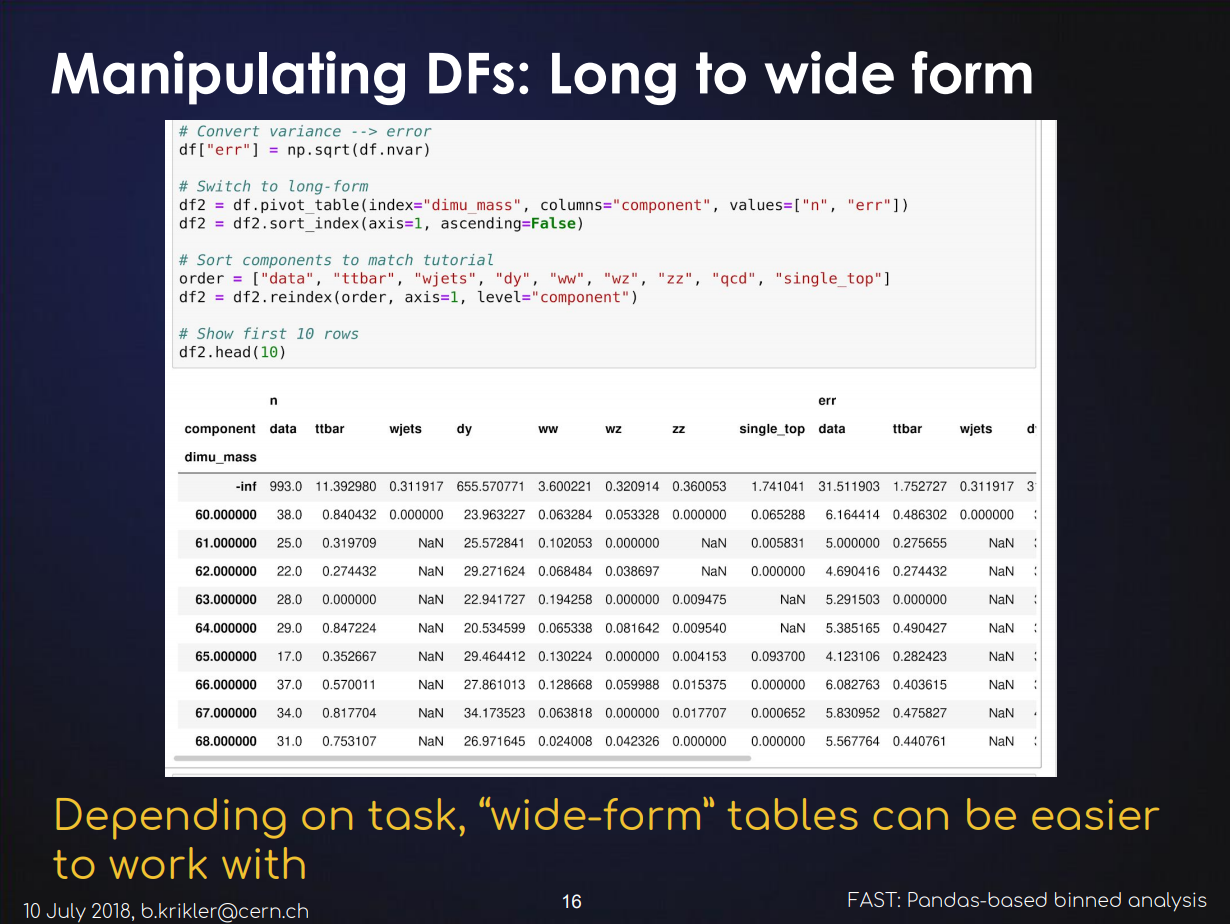
\includegraphics[width=0.75\linewidth]{fast-slide-2.png}}
\end{center}
\end{frame}

\begin{frame}[fragile]{Indexed analysis}
\vspace{0.1 cm}
\begin{columns}
\column{1.09\linewidth}
\begin{onlyenv}<1-2>Booking/filling mechanism with tree-like semantic index:

\hfill 
\includegraphics[height=1 cm]{histbook-logo.pdf}

\vspace{-1 cm}
\scriptsize
\begin{minted}{python}
>>> from histbook import *
>>> histograms = \
...     ChannelsBook(
...         mass = SamplesBook(["data", "signal", "background"],
...                   SystematicsBook(Hist(bin("x", 5, 0, 5), systematic=[0]),
...                                   Hist(bin("x + epsilon", 5, 0, 5), systematic=[1]),
...                                   Hist(bin("x - epsilon", 5, 0, 5), systematic=[-1]))),
...         mctruth = SamplesBook(["signal", "background"],
...                         Book(param1=Hist(bin("param1", 5, 0, 5)),
...                              param2=Hist(bin("param2", 5, 0, 5)))))
\end{minted}

\normalsize
defines $3\times 3 + 2\times2$ histograms and verifies that binning matches for systematic variations.

\scriptsize
\begin{uncoverenv}<2->
\begin{minted}{python}
>>> histograms.allkeys()
['mass', 'mass/data', 'mass/data/0', 'mass/data/0/0', 'mass/data/0/1', 'mass/data/0/2',
 'mass/signal', 'mass/signal/0', 'mass/signal/0/0', 'mass/signal/0/1', 'mass/signal/0/2',
 'mass/background', 'mass/background/0', 'mass/background/0/0',  'mass/background/0/1',
 'mass/background/0/2', 'mctruth', 'mctruth/signal', 'mctruth/signal/0',
 'mctruth/signal/0/param2', 'mctruth/signal/0/param1', 'mctruth/background',
 'mctruth/background/0', 'mctruth/background/0/param2', 'mctruth/background/0/param1']
\end{minted}
\end{uncoverenv}
\vspace{-0.7 cm}
\end{onlyenv}
\begin{onlyenv}<3>
\scriptsize
\begin{minted}{python}
>>> print(histograms["mass"])                   # print just the "mass" channel
SamplesBook({
    'data': Book({
          '0': SystematicsBook({
                '0': Hist(bin('x', 5, 0.0, 5.0)),
                '1': Hist(bin('x + epsilon', 5, 0.0, 5.0)),
                '2': Hist(bin('x - epsilon', 5, 0.0, 5.0))
                })
          }),
    'signal': Book({
          '0': SystematicsBook({
                '0': Hist(bin('x', 5, 0.0, 5.0)),
                '1': Hist(bin('x + epsilon', 5, 0.0, 5.0)),
                '2': Hist(bin('x - epsilon', 5, 0.0, 5.0))
                })
          }),
    'background': Book({
          '0': SystematicsBook({
                '0': Hist(bin('x', 5, 0.0, 5.0)),
                '1': Hist(bin('x + epsilon', 5, 0.0, 5.0)),
                '2': Hist(bin('x - epsilon', 5, 0.0, 5.0))
                })
          })})
\end{minted}
\end{onlyenv}
\begin{onlyenv}<4>
\scriptsize
\begin{minted}{python}
>>> print(histograms.view("*/signal/*"))        # select the subtree matching this pattern
ViewBook({
      'mass': ViewBook({
            'signal': ViewBook({
                  '0': ViewBook({
                        '0': Hist(bin('x', 5, 0.0, 5.0)),
                        '1': Hist(bin('x + epsilon', 5, 0.0, 5.0)),
                        '2': Hist(bin('x - epsilon', 5, 0.0, 5.0))
                        })
                  })
            }),
      'mctruth': ViewBook({
            'signal': ViewBook({
                  '0': ViewBook({
                        'param2': Hist(bin('param2', 5, 0.0, 5.0)),
                        'param1': Hist(bin('param1', 5, 0.0, 5.0))
                        })
                  })
            })
      })
>>> histograms.view("*/data/*").fill(data)      # fill selectively
>>> histograms.view("*/signal/*").fill(signal)
>>> histograms.view("*/background/*").fill(background)
\end{minted}
\end{onlyenv}
\end{columns}
\end{frame}

\begin{frame}{Indexed analysis}
\Large
\vspace{0.5 cm}
Using tools with rich indexing systemizes what we're doing with naming conventions, splitting histogram names on underscores, etc.

\vspace{1 cm}
Pandas is not a TTree replacement--- if anything, it's a histogram organizer!
\end{frame}

\begin{frame}{Advanced histogramming}
\large
\vspace{0.5 cm}
{\Large The histograms themselves, however, are more sophisticated in HEP than elsewhere.}
\vspace{0.25 cm}
\begin{itemize}\setlength{\itemsep}{0.25 cm}
\item<2-> As far as I have found, HEP histogramming tools (ROOT, YODA, AIDA, HippoDraw, Jas3, mn\_fit, PAW, HBOOK) are \underline{\it unique} in conceiving of a histogram as a container to be filled, merged, and accessed programmatically.
\item<3-> In many non-HEP packages, ``histogram'' is more of a display option than an analysis tool, with no way to access contents or control binning.
\item<4-> Only HEP tools have ``profile'' histograms--- functions of dependent variables, in addition to distributions on independent variables.
\item<5-> Log-scale support is often weak in non-HEP graphics packages, particularly for empty bins.
\end{itemize}
\begin{center}
\uncover<6->{\textcolor{red}{These features aren't difficult: but they're our responsibility.}}
\end{center}
\end{frame}

\begin{frame}{Machine learning versus ansatz fitting}
\end{frame}




\end{document}
